% -*- latex -*-
%%%%%%%%%%%%%%%%%%%%%%%%%%%%%%%%%%%%%%%%%%%%%%%%%%%%%%%%%%%%%%%%
%%%%%%%%%%%%%%%%%%%%%%%%%%%%%%%%%%%%%%%%%%%%%%%%%%%%%%%%%%%%%%%%
%%%%
%%%% This text file is part of the source of 
%%%% `Parallel Programming in MPI and OpenMP'
%%%% by Victor Eijkhout, copyright 2012-2022
%%%%
%%%% petsc-fem.tex : FEM through DMPLEX
%%%%
%%%%%%%%%%%%%%%%%%%%%%%%%%%%%%%%%%%%%%%%%%%%%%%%%%%%%%%%%%%%%%%%
%%%%%%%%%%%%%%%%%%%%%%%%%%%%%%%%%%%%%%%%%%%%%%%%%%%%%%%%%%%%%%%%

\Level 0 {General Data Management}

\cverbatimsnippet{pdmcreate}

A \indexpetscshow{DMPLEX} is by default two-dimensional.
Use
\begin{verbatim}
plexprogram  -dm_plex_dim k
\end{verbatim}
for other dimensions.
In two dimensions there are three levels of cells:
\begin{itemize}
\item
  0-cells are vertices,
\item 1-cells are edges, and
\item 2-cells are triangles.
\end{itemize}

The default $2\times 2$ grid has, sequentially:
\csnippetwithoutput{pdmview}{code/petsc/c}{sphereviewnp1}
and parallel:
\csnippetwithoutput{pdmview}{code/petsc/c}{sphereviewnp4}

For larger grids:
\begin{verbatim}
plexprogram -dm_plex_box_faces 4,4
\end{verbatim}

\begin{multicols}{2}
  Graphics output from
\begin{verbatim}
plexprogram -dm_view draw -draw_pause 20
\end{verbatim}
\vfill\hbox{}
\columnbreak
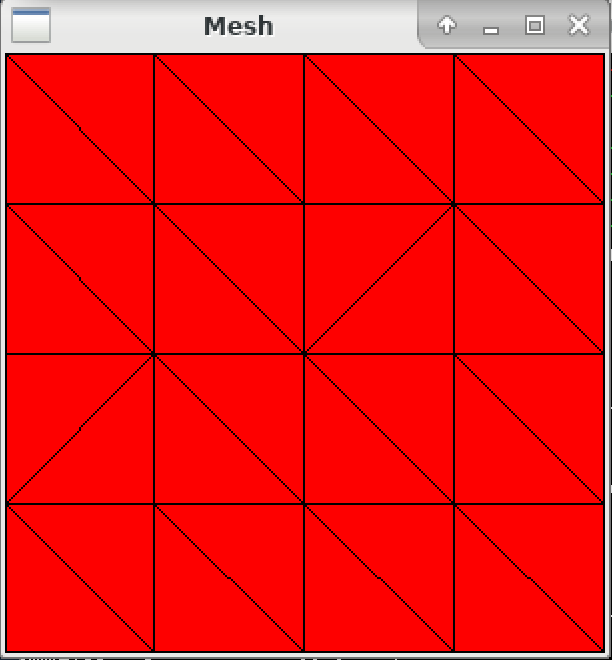
\includegraphics[scale=.5]{dmplex4x4}
\end{multicols}

\begin{verbatim}
plexprogram -dm_view :outputfile.tex:ascii_latex \
            -dm_plex_view_scale 4
\end{verbatim}

\hbox to \textwidth {
\input mesh-plex7-p1.tex
\hfil
\input mesh-plex7-p2.tex
}

\Level 1 {Matrix from dmplex}

\begin{tabbing}
  Loop \=over batch of elements (e):\\
  \>Loop \=over element matrix entries (f,fc,g,gc --> i,j:\\
  \>\>Loop \=over quadrature points (q):\\
  \>\>\>Make \n{u_q} and \n{gradU_q} (loops over fields,Nb,Ncomp)\\
  \>\>\> \n{elemMat[i,j] +=} \= $\psi^{fc}_f(q) g^{(0)}_{fc,gc}(u, \nabla u) \phi^{gc}_g(q)$\\
  \>\>\>\> $+ \psi^{fc}_f(q) \cdot g^{(1)}w_{fc,gc,dg}(u, \nabla u) \nabla\phi^{gc}_g(q)$\\
  \>\>\>\> $+ \nabla\psi^{fc}_f(q) \cdot g^{(2)}_{fc,gc,df}(u, \nabla u) \phi^{gc}_g(q)$\\
  \>\>\>\> $+ \nabla\psi^{fc}_f(q) \cdot g^{(3)}_{fc,gc,df,dg}(u, \nabla u) \nabla\phi^{gc}_g(q)$\\
\end{tabbing}

\cverbatimsnippet{psectionsetup}
%% \begin{lstlisting}
%%   ierr = DMPlexGetDepthStratum(dm, 0, &vStart, &vEnd);CHKERRQ(ierr);
%%   ierr = PetscSectionCreate(PetscObjectComm((PetscObject) dm), &s);CHKERRQ(ierr);
%%   // setup the section
%%   ierr = DMSetLocalSection(dm, s);CHKERRQ(ierr);
%%   ierr = PetscSectionDestroy(&s);CHKERRQ(ierr);
%% \end{lstlisting}

\cverbatimsnippet{psectionloop}
%% \begin{lstlisting}
%%   ierr = PetscSectionSetNumFields(s, 1);CHKERRQ(ierr);
%%   ierr = PetscSectionSetFieldComponents(s, 0, 1);CHKERRQ(ierr);
%%   ierr = PetscSectionSetChart(s, vStart, vEnd);CHKERRQ(ierr);
%%   //  printf("start-end: %d -- %d\n",vStart,vEnd);
%%   for (v = vStart; v < vEnd; ++v) {
%%     ierr = PetscSectionSetDof(s, v, 1);CHKERRQ(ierr);
%%     ierr = PetscSectionSetFieldDof(s, v, 0, 1);CHKERRQ(ierr);
%%   }
%%   ierr = PetscSectionSetUp(s);CHKERRQ(ierr);
%% \end{lstlisting}

\endinput

\begin{lstlisting}
PetscDSSetJacobian
Set the pointwise Jacobian function for given test and basis fields
Synopsis

#include "petscds.h" 
PetscErrorCode PetscDSSetJacobian(PetscDS prob, PetscInt f, PetscInt g,
    void (*g0)(PetscInt dim, PetscInt Nf, PetscInt NfAux,
        const PetscInt uOff[], const PetscInt uOff_x[], const PetscScalar u[], const PetscScalar u_t[], const PetscScalar u_x[],
        const PetscInt aOff[], const PetscInt aOff_x[], const PetscScalar a[], const PetscScalar a_t[], const PetscScalar a_x[],
        PetscReal t, PetscReal u_tShift, const PetscReal x[], PetscInt numConstants, const PetscScalar constants[], PetscScalar g0[]),
    void (*g1)(PetscInt dim, PetscInt Nf, PetscInt NfAux,
        const PetscInt uOff[], const PetscInt uOff_x[], const PetscScalar u[], const PetscScalar u_t[], const PetscScalar u_x[],
        const PetscInt aOff[], const PetscInt aOff_x[], const PetscScalar a[], const PetscScalar a_t[], const PetscScalar a_x[],
        PetscReal t, PetscReal u_tShift, const PetscReal x[], PetscInt numConstants, const PetscScalar constants[], PetscScalar g1[]),
    void (*g2)(PetscInt dim, PetscInt Nf, PetscInt NfAux,
        const PetscInt uOff[], const PetscInt uOff_x[], const PetscScalar u[], const PetscScalar u_t[], const PetscScalar u_x[],
        const PetscInt aOff[], const PetscInt aOff_x[], const PetscScalar a[], const PetscScalar a_t[], const PetscScalar a_x[],
        PetscReal t, PetscReal u_tShift, const PetscReal x[], PetscInt numConstants, const PetscScalar constants[], PetscScalar g2[]),
    void (*g3)(PetscInt dim, PetscInt Nf, PetscInt NfAux,
        const PetscInt uOff[], const PetscInt uOff_x[], const PetscScalar u[], const PetscScalar u_t[], const PetscScalar u_x[],
        const PetscInt aOff[], const PetscInt aOff_x[], const PetscScalar a[], const PetscScalar a_t[], const PetscScalar a_x[],
        PetscReal t, PetscReal u_tShift, const PetscReal x[], PetscInt numConstants, const PetscScalar constants[], PetscScalar g3[])
)
\end{lstlisting}

\[
\int_\Omega \phi g_0(u, u_t, \nabla u, x, t) \psi + \phi {\vec g}_1(u, u_t, \nabla u, x, t) \nabla \psi + \nabla\phi \cdot {\vec g}_2(u, u_t, \nabla u, x, t) \psi + \nabla\phi \cdot {\overleftrightarrow g}_3(u, u_t, \nabla u, x, t) \cdot \nabla \psi
\]
